% Quarto/Pandoc template for the MDPI class (Remote Sensing)
% Generated for ARTICLE_NDVI_V10_A3_MDPI.qmd
\documentclass[remotesensing,article,submit,pdftex,oneauthor]{Definitions/mdpi}

\firstpage{1}
\makeatletter
\setcounter{page}{\@firstpage}
\makeatother
\pubvolume{1}
\issuenum{1}
\articlenumber{0}
\pubyear{2026}
\copyrightyear{2026}
\datereceived{}
\daterevised{}
\dateaccepted{}
\datepublished{}

% Packages required by Pandoc output but not loaded by mdpi.cls
\usepackage{longtable}
\usepackage{fancyvrb}
\usepackage{framed}
\usepackage{fvextra}
\usepackage{textcomp}
\usepackage{upquote}
\setkeys{Gin}{keepaspectratio}


% CLEAN_PREPUBLICATION_PAGE_STYLE_V13
% Retain the MDPI manuscript layout while suppressing the class-generated
% placeholder DOI and automatic submission-date text.
\makeatletter

\fancypagestyle{plain}{%
  \fancyhf{}%
  \fancyfoot[C]{%
    \fontsize{8}{8}\selectfont
    \thepage\ of \pageref*{LastPage}%
  }%
}

\pagestyle{fancy}
\fancyhf{}

\fancyhead[R]{%
  \fontsize{8}{8}\selectfont
  \thepage\ of \pageref*{LastPage}%
}

\lhead{}
\chead{}
\rfoot{}
\cfoot{}
\lfoot{}

\makeatother

% Pandoc compatibility
\providecommand{\tightlist}{%
  \setlength{\itemsep}{0pt}\setlength{\parskip}{0pt}}
\providecommand{\pandocbounded}[1]{#1}
\newcommand{\passthrough}[1]{#1}


% CSL compatibility (normally unused because natbib is selected)
\newlength{\cslhangindent}
\setlength{\cslhangindent}{1.5em}
\newlength{\csllabelwidth}
\setlength{\csllabelwidth}{3em}
\newenvironment{CSLReferences}[2]
 {\begin{list}{}{
   \setlength{\itemindent}{0pt}
   \setlength{\leftmargin}{0pt}
   \setlength{\parsep}{0pt}
   \ifodd #1
     \setlength{\leftmargin}{\cslhangindent}
     \setlength{\itemindent}{-1\cslhangindent}
   \fi}}
 {\end{list}}
\newcommand{\CSLBlock}[1]{#1\hfill\break}
\newcommand{\CSLLeftMargin}[1]{\parbox[t]{\csllabelwidth}{#1}}
\newcommand{\CSLRightInline}[1]{\parbox[t]{\dimexpr\linewidth-\csllabelwidth\relax}{#1}\break}
\newcommand{\CSLIndent}[1]{\hspace{\cslhangindent}#1}

% Metadata
\Title{Category-Specific Sentinel-2 NDVI Differences among Level-1C,
Sen2Cor, and LaSRC in a Tropical Silvopastoral Landscape}
\Author{Heiber Alexander Pantevez Villamil $^{1,2,}$*\orcidA{}}
\AuthorNames{Heiber Alexander Pantevez Villamil}
\address{$^{1}$ \quad Doctoral Program in Agroecology, Facultad de Ciencias Agropecuarias, Universidad Nacional de Colombia, Sede Palmira, Palmira, Colombia\\ $^{2}$ \quad Facultad de Ciencias Agrarias, Universidad Nacional de Colombia, Sede Bogot\'{a}, Bogot\'{a}, Colombia (internal mobility)}
\corres{\textbf{*} \quad Correspondence: hapantevezv@unal.edu.co}
\newcommand{\orcidauthorA}{0000-0003-1797-0057}
\abstract{Consistency among Sentinel-2 processing levels is essential
when normalized difference vegetation index (NDVI) time series combine
top-of-atmosphere (TOA) and surface-reflectance (SR) products. We
quantified paired NDVI differences among Level-1C/TOA, Sen2Cor L2A/SR,
and LaSRC L2A/SR for 106 land-use management polygons on 22 farms in the
Colombian Orinoco Piedmont. Acquisitions from 2019-2020 were matched by
date and polygon. Local L1C and LaSRC observations were screened with
Fmask 4.6 and s2cloudless, and Sen2Cor observations with the Scene
Classification Layer. Across 1,797 common observations, mean differences
were +0.116 for LaSRC-L1C (95\% farm-cluster bootstrap CI, 0.108 to
0.124; RMSD = 0.121; CCC = 0.653; Deming slope = 1.092; 95\% limits of
agreement, 0.047 to 0.184) and +0.095 for Sen2Cor-L1C (0.086 to 0.101;
RMSD = 0.101; CCC = 0.743; slope = 1.155; limits, 0.027 to 0.162). LaSRC
and Sen2Cor agreed more closely (mean difference = +0.021; RMSD = 0.036;
CCC = 0.962; slope = 0.945, CI 0.916 to 0.972; limits, -0.035 to 0.078),
with nearly identical mean differences in 2019 and 2020. TOA-SR
differences were largest for secondary forest or wetlands undergoing
restoration and smallest for other agricultural practices. On 2,585
paired records, masking changed neither the mean difference (+0.0001;
CI, -0.0021 to 0.0024) nor CCC (+0.0014; -0.0078 to 0.0146)
distinguishably from zero, but increased the Deming slope by +0.0191
(0.0028 to 0.0312). Sentinel-2 NDVI differences were therefore
processor- and land-use-dependent, supporting explicit harmonization
when TOA and SR observations are combined.}
\keyword{Sentinel-2 MSI; surface
reflectance; Sen2Cor; LaSRC; NDVI; tropical silvopastoral
systems; method comparison}

\begin{document}

\section{Introduction}\label{sec-intro}

Radiometric consistency is fundamental to the interpretation of
vegetation-index time series derived from Sentinel-2 MSI
\citep{Drusch2012}. Conversion from Level-1C top-of-atmosphere (TOA)
reflectance to Level-2A surface reflectance (SR) changes the red and
near-infrared signals used to calculate NDVI because atmospheric
correction responds to aerosol optical thickness, water vapour,
illumination-view geometry, and surface spectral properties
\citep{Doxani2018, Martins2017, Marujo2021}. These effects are
particularly relevant in humid tropical environments, where persistent
cloud, cirrus, and high atmospheric water vapour complicate the
construction of radiometrically consistent multi-year series
\citep{Chraibi2022}.

Sen2Cor and LaSRC are two established routes for generating Sentinel-2
SR products. Sen2Cor is the European Space Agency Level-2A processor
distributed through the Copernicus ecosystem
\citep{MainKnorn2017, ESA2026Sen2Cor}. LaSRC was developed for Landsat
and subsequently adapted for Sentinel-2; it is also the
atmospheric-correction component used in the Harmonized Landsat
Sentinel-2 workflow \citep{Vermote2016, Vermote2018, Claverie2018}.
Previous intercomparisons have evaluated atmospheric-correction products
over forests, inland waters, and AERONET sites
\citep{Martins2017, Marujo2021, Chraibi2022}, but evidence remains
limited for heterogeneous tropical landscapes in which pastures, trees,
restoration areas, and agricultural uses coexist within short distances.

This study addresses processor-associated NDVI differences in a
spatially clustered network of land-use management polygons in the
Piedemonte Orinocense transition zone, with three specific objectives
for the complete 2019-2020 observation period: (i) to quantify the
magnitude and structure of paired NDVI differences among L1C/TOA,
Sen2Cor L2A/SR, and LaSRC L2A/SR; (ii) to characterize how these
differences vary across the six Sustainable Cattle Ranching (SCR)
land-use categories represented in the analytical sample; and (iii) to
evaluate how Fmask+s2cloudless screening of LaSRC observations affects
paired agreement with SCL-screened Sen2Cor observations.

The study quantifies agreement and processor-associated differences
rather than absolute accuracy, because no co-located field or
atmospheric reference was available to identify which product was
closest to true surface NDVI.

\section{Study Area and Data}\label{sec-area}

\subsection{Study Area}\label{sec-study-area}

The area of interest is located in the Colombian Orinoco Piedmont
(\emph{Piedemonte Orinocense}), Department of Meta, Colombia, an
ecological and biogeographic transition belt between the eastern
foothills of the Cordillera Oriental and the Llanos Orientales plains.
It comprises 22 farms with a combined mapped area of 854 ha across
Granada, Fuente de Oro, San Juan de Arama, and El Castillo
(Figure~\ref{fig-study-area}). For these farms, the 2019 vector
inventory contains 143 management-polygon features, which together cover
the mapped farm area and define 141 management polygons identified by
farm, polygon, and land-use code; these polygons constitute the spatial
units of analysis. The farms intersect the adjacent Sentinel-2 MGRS
tiles 18NXJ and 18NXK in UTM zone 18N. Overlay of the management
polygons with the IDEAM continental ecosystems map
\citep{IDEAM2017Ecosistemas} shows that polygon area is dominated by the
Alternating-Hygric Tropical Zonobiome (\emph{Zonobioma Alternohígrico
Tropical}; 66.3\%), with smaller contributions from the Humid Tropical
Zonobiome (13.7\%) and the Subandean Orobiome (9.5\%). Consistent with a
long-transformed silvopastoral landscape rather than an open-savanna
setting, the IDEAM 2020 land-cover layer \citep{IDEAM2020Coberturas}
classifies only 0.5\% of polygon area as natural grassland, while 66.6\%
corresponds to managed pasture and 7.9\% to forest cover. All valid
acquisitions matched across the processing pipelines during 2019 and
2020 were included, without restriction to a seasonal or phenological
window.

The polygon inventory was produced within the Sustainable Cattle
Ranching project (SCR; \emph{Proyecto Ganadería Colombiana Sostenible}),
an institutional partnership involving FEDEGÁN-FNG, CIPAV, Fondo Acción,
The Nature Conservancy, and the World Bank
\citep{SCROperationalManual2014, SCR2019Inventory}.

\begin{figure}[htbp]

\centering{

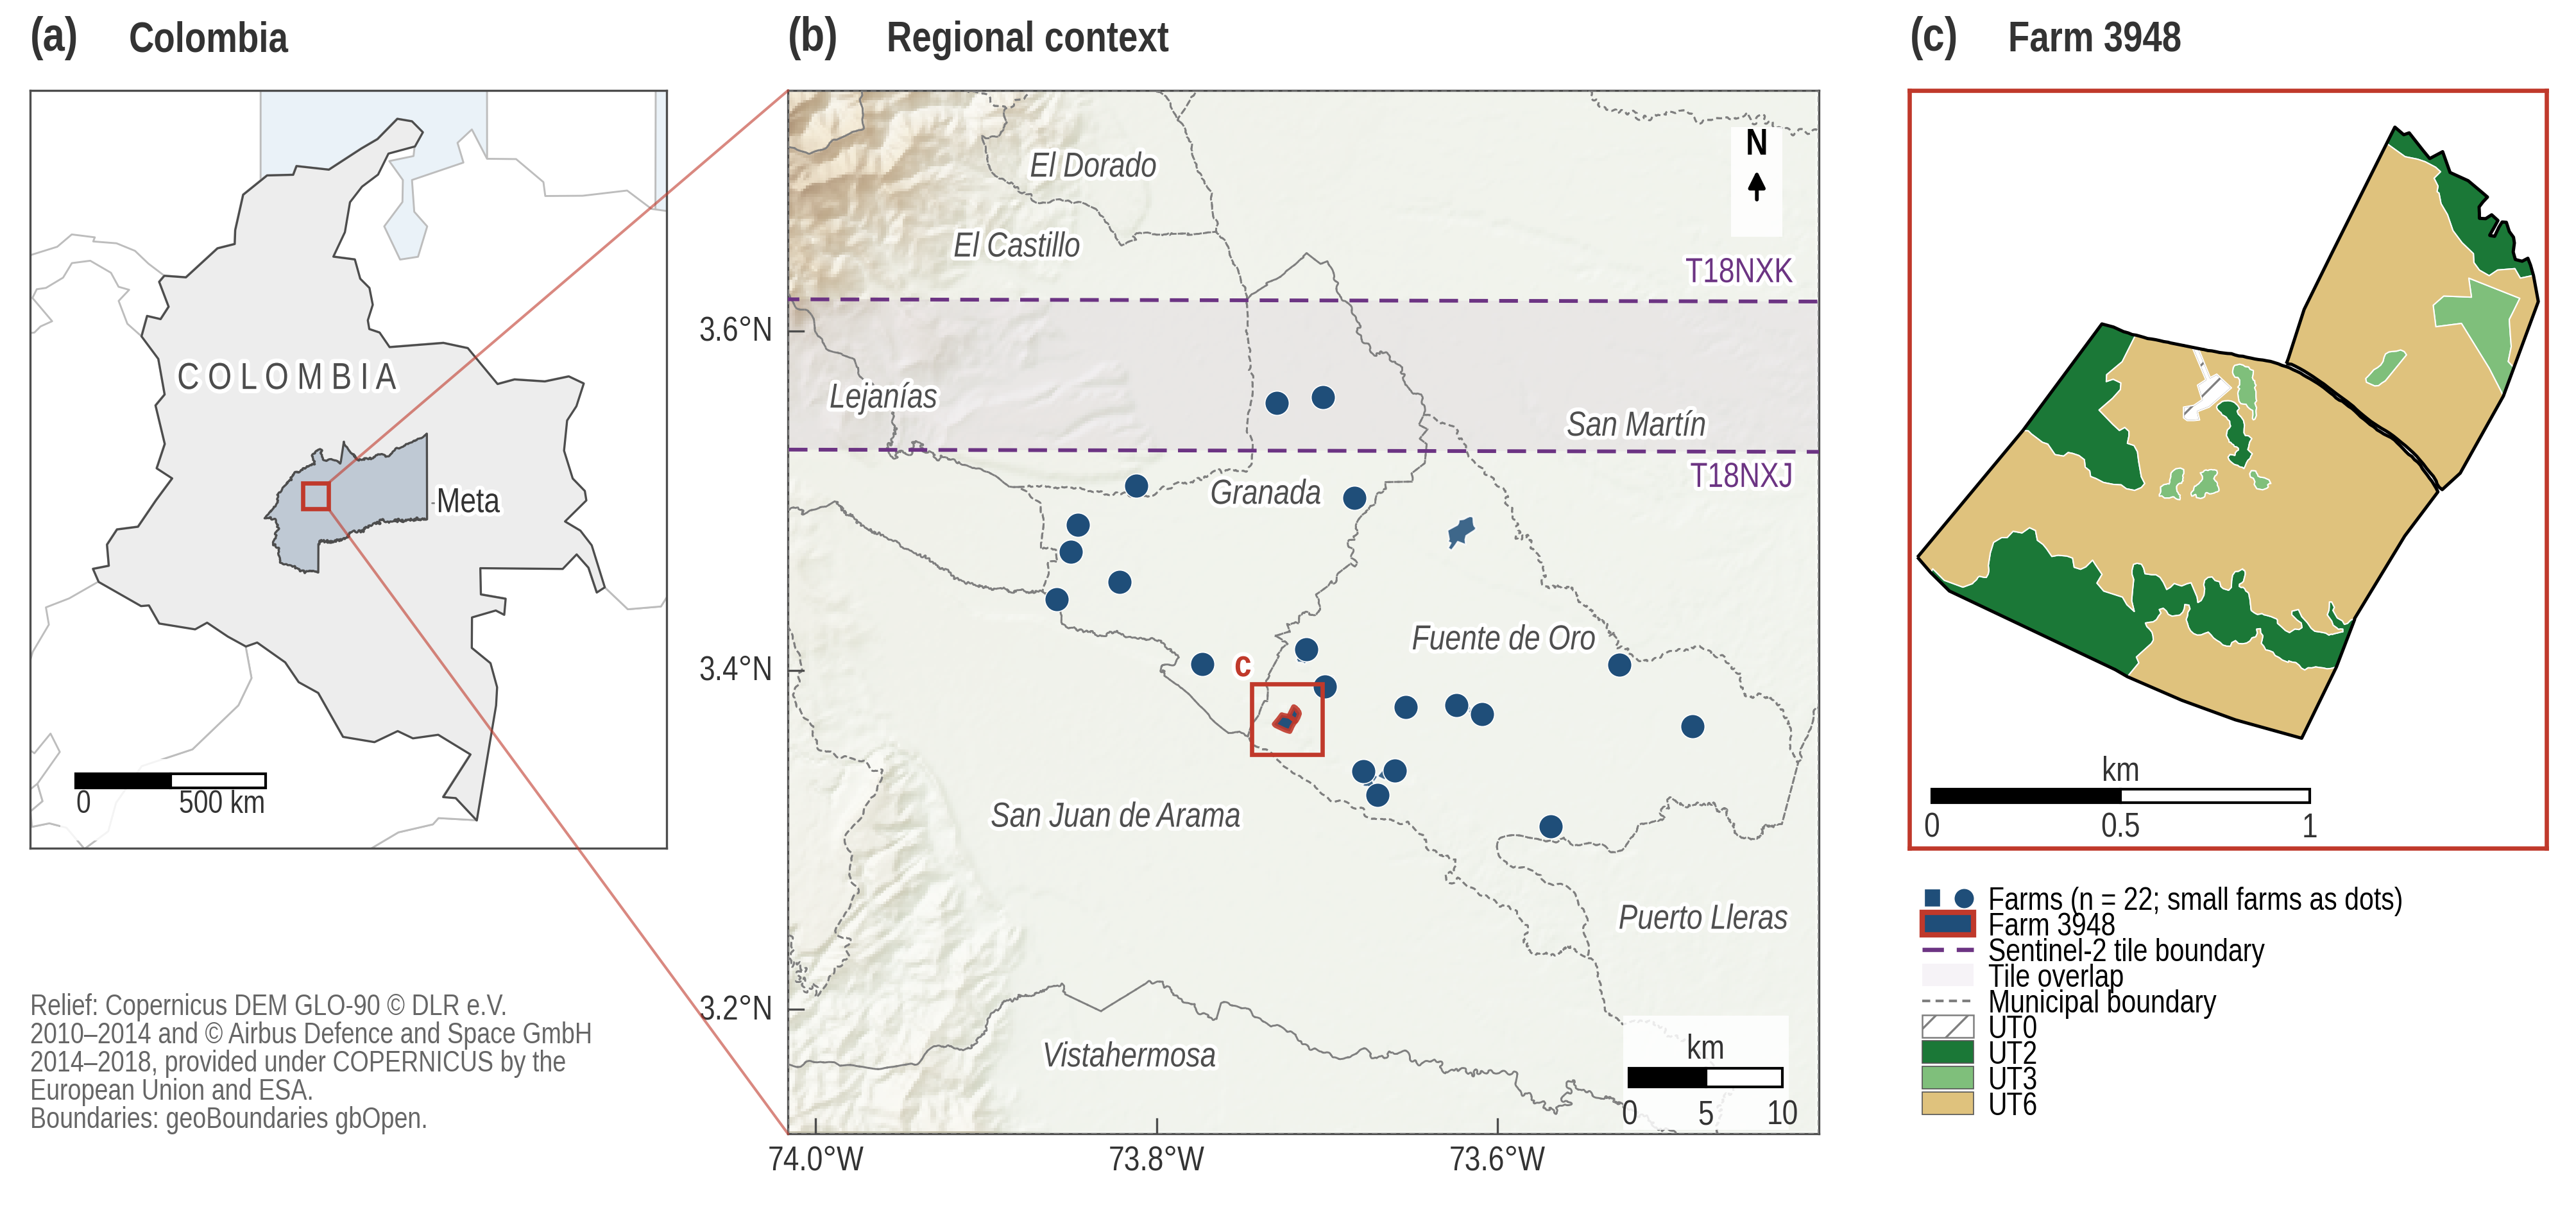
\includegraphics[width=1\textwidth,height=\textheight]{figures/figure_01_study_area.png}

}

\caption{\label{fig-study-area}Study area in the Orinoco Piedmont,
Department of Meta, Colombia. (a) Location in Colombia. (b) The 22 farms
(small farms shown as dots), municipal boundaries, and Sentinel-2 tiles
18NXJ and 18NXK (shaded: tile overlap) over shaded relief. (c)
Management polygons of farm 3948 (red box in b; shown in
Figure~\ref{fig-three-pipelines}) by SCR land-use category
(Table~\ref{tbl-ut}). Relief: Copernicus DEM GLO-90.}

\end{figure}%

\subsection{SCR Land-Use Categories}\label{sec-ut}

Land-use codes follow the official SCR land-use manual
\citep{SCRLandUseManual2017}. The category-stratified analysis included
the six categories represented in the common three-pipeline dataset
(Table~\ref{tbl-ut}); English translations are used throughout the
results and discussion, and original Spanish category labels are omitted
here for brevity.

\begin{longtable}[]{@{}cl@{}}
\caption{Official SCR land-use categories represented in the analysis
\citep{SCRLandUseManual2017}.}\label{tbl-ut}\tabularnewline
\toprule\noalign{}
Code & Land-use category \\
\midrule\noalign{}
\endfirsthead
\toprule\noalign{}
Code & Land-use category \\
\midrule\noalign{}
\endhead
\bottomrule\noalign{}
\endlastfoot
UT2 & Secondary forest or wetlands undergoing restoration \\
UT3 & Scattered trees in pasture and vegetative succession \\
UT4 & Agroforestry crops \\
UT6 & Agricultural land with vegetation cover greater than 80\% \\
UT7 & Intensive silvopastoral system \\
UT8 & Other agricultural practices \\
\end{longtable}

\subsection{Analytical Dataset}\label{sec-inclusion}

The observational unit was a polygon-by-date record. The polygon
identifier combined the farm identifier, the polygon number, and the SCR
land-use code. A record entered the three-pipeline comparison when the
same acquisition date and polygon identifier were present for L1C,
Sen2Cor, and LaSRC, and when the locally processed L1C and LaSRC
observations each contained at least 10 valid 10 m pixels after
Fmask+s2cloudless screening. Polygon-by-date records that remained
duplicated within a pipeline, because two inventory features shared the
same identifier, were excluded rather than averaged. Exact matching
yielded 1,810 records; one record was removed during cross-product
quality control (Section~\ref{sec-statistics}), and 12 records failed
the valid-pixel threshold in the LaSRC pipeline. The common
three-pipeline dataset therefore comprised 1,797 polygon-by-date records
from 106 management polygons on 22 farms (668 records in 2019 and 1,129
in 2020).

The land-use analysis comprised the 1,527 common records from 88
management polygons on 21 farms assigned to the six SCR categories in
Table~\ref{tbl-ut}. The masking-sensitivity analysis used the 2,585
polygon-by-date records (128 polygons, 20 farms) present in both the
masked and unmasked LaSRC exports and paired with the same SCL-screened
Sen2Cor observations; a stricter subset of 2,521 records with at least
10 valid pixels in both LaSRC exports was analysed as a sensitivity
check.

\section{Materials and Methods}\label{sec-methods}

\begin{figure}[htbp]

\centering{

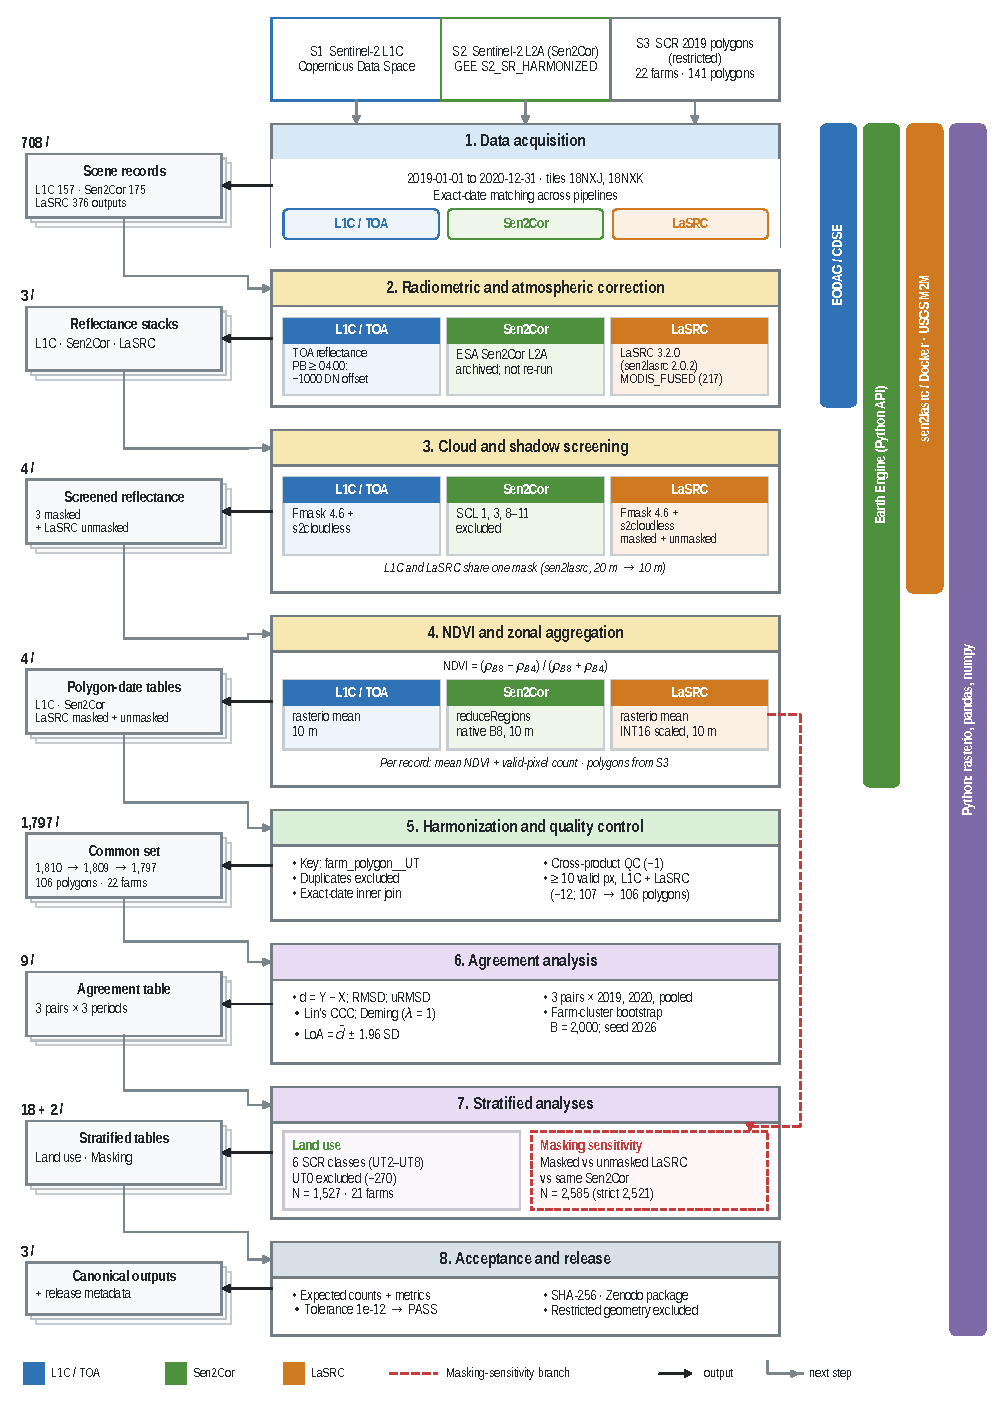
\includegraphics[width=0.9\textwidth,height=\textheight]{figures/figure_02_processing_workflow.pdf}

}

\caption{\label{fig-method-workflow}Processing and analysis workflow.
The central column lists the processing steps (1--8), the left column
the products of each step with their size, and the right column the
software used. S1--S3 are the data sources. Colours identify the three
processing pipelines (blue, L1C/TOA; green, Sen2Cor; orange, LaSRC); L1C
and LaSRC share one Fmask + s2cloudless mask. The dashed red path marks
the masking-sensitivity analysis, which pairs masked and unmasked LaSRC
exports with the same Sen2Cor records. All counts correspond to the
canonical analysis that passed the acceptance tests.}

\end{figure}%

\subsection{Processing Pipelines}\label{sec-processing}

The comparison held acquisition date, polygon identifier, B8/B4 NDVI
formulation, and a 10 m target resolution constant across the three
pipelines. Atmospheric correction, pixel-quality screening, processing
platform, and zonal-aggregation implementation differed among pipelines
and are therefore part of the processing-chain effect evaluated in this
study.

\textbf{L1C/TOA pipeline.} Sentinel-2 Level-1C images for tiles 18NXJ
and 18NXK were retrieved from the Copernicus Data Space Ecosystem with
EODAG 3.10.2. Scenes were pre-screened using
\texttt{CLOUDY\_PIXEL\_PERCENTAGE\ \textless{}=\ 20}. For products with
Processing Baseline 04.00 or later, the 1000-DN offset was removed
before reflectance scaling, thereby maintaining consistency with
harmonized Sentinel-2 collections \citep{GEE2026S2SR}. NDVI was
calculated from B8 (near infrared, 10 m) and B4 (red, 10 m).

\textbf{Sen2Cor L2A/SR pipeline.} Sen2Cor-derived SR was obtained from
\texttt{COPERNICUS/S2\_SR\_HARMONIZED} through the Google Earth Engine
Python API for acquisitions between 1 January 2019 and 31 December 2020.
The collection harmonizes digital-number ranges across Sentinel-2
processing baselines \citep{GEE2026S2SR}. For each target date of the
local inventory, the least cloudy image within a short search window was
selected; all 175 selected images coincided exactly with the target
acquisition date. Because the archive does not expose a local executable
version for each image, the results refer to the harmonized collection
rather than to a single locally executed Sen2Cor release. Zonal
statistics were calculated on the native B8 projection at 10 m.

\textbf{LaSRC L2A/SR pipeline.} The corresponding L1C acquisitions were
processed with \texttt{sen2lasrc} v2.0.2, which executes LaSRC 3.2.0 and
integrates EODAG, Fmask, and s2cloudless in a Docker workflow
\citep{deBoissieu2024, Qiu2019, SentinelHubS2Cloudless}. The processing
image was the \texttt{lasrc-fmask} image of the \texttt{sen2lasrc}
project, pinned by its SHA-256 digest (\texttt{14fcc58ac2bd…}; the full
digest is recorded in \texttt{environment/container-provenance.txt} and
in the Zenodo deposit). MODIS-based fused atmospheric auxiliary data
(MODIS\_FUSED) for 2019-2020 were retrieved through the USGS
Machine-to-Machine (M2M) API \citep{USGS2026M2M}. Surface reflectance
was stored as scaled \texttt{INT16}; pixels assigned the product no-data
value were removed before NDVI calculation.

\subsection{Cloud and Shadow Screening}\label{sec-masks}

Sen2Cor observations were screened with the Scene Classification Layer
(SCL). Classes 1 (saturated or defective), 3 (cloud shadow), 8 and 9
(medium- and high-probability cloud), 10 (thin cirrus), and 11 (snow or
ice) were excluded; pixels without valid reflectance (class 0, no data)
carry no valid B4 or B8 values in the Earth Engine collection and
therefore did not contribute to the zonal statistics. The local L1C and
LaSRC pipelines shared the same pixel mask: Fmask 4.6 and s2cloudless
layers were generated once by \texttt{sen2lasrc} at 20 m, resampled to
the 10 m analysis grid, and applied identically to both pipelines,
retaining pixels classified as clear land by Fmask and as cloud-free by
s2cloudless. The only masking asymmetry in the three-pipeline comparison
was therefore between this shared mask and the Sen2Cor SCL screening.
Consequently, the observed inter-pipeline differences combine the
effects of atmospheric correction with residual differences in masking,
rasterization, and zonal aggregation. The paired masking analysis
isolates the effect of LaSRC screening on a fixed set of polygon-by-date
observations.

\subsection{Angular and BRDF Considerations}\label{sec-angular}

No normalization to a common bidirectional reflectance distribution
function (BRDF) geometry was applied, although Sentinel-2 reflectance
shows measurable directional effects across the swath \citep{Roy2017}.
LaSRC atmospheric correction is distinct from the NBAR/BRDF
normalization subsequently applied in the HLS product
\citep{Franch2019, Ju2025HLS, USGSHLS2024}. Solar zenith angles in the
archived L1C metadata were approximately 25-38 degrees and view zenith
angles approximately 0-9 degrees; residual illumination-view effects may
therefore contribute to the observed differences.

\subsection{NDVI Calculation and Zonal
Aggregation}\label{sec-aggregation}

NDVI was calculated pixel-wise as

\[
\mathrm{NDVI}=\frac{\rho_{B8}-\rho_{B4}}{\rho_{B8}+\rho_{B4}}.
\]

For each polygon-by-date record, mean NDVI was the primary statistic;
median, standard deviation, and valid-pixel count were retained for
quality control. Local L1C and LaSRC statistics were calculated with
\texttt{rasterio.mask}. Sen2Cor statistics were calculated with Google
Earth Engine \texttt{reduceRegions} using the native B8 projection and a
10 m scale.

\subsection{Pairwise Differences}\label{sec-differences}

Pairwise differences were defined as

\[
\Delta\mathrm{NDVI}_{\mathrm{LaSRC-L1C}}=\mathrm{NDVI}_{\mathrm{LaSRC}}-\mathrm{NDVI}_{\mathrm{L1C}},
\]

\[
\Delta\mathrm{NDVI}_{\mathrm{Sen2Cor-L1C}}=\mathrm{NDVI}_{\mathrm{Sen2Cor}}-\mathrm{NDVI}_{\mathrm{L1C}},
\]

and

\[
\Delta\mathrm{NDVI}_{\mathrm{LaSRC-Sen2Cor}}=\mathrm{NDVI}_{\mathrm{LaSRC}}-\mathrm{NDVI}_{\mathrm{Sen2Cor}}.
\]

Positive values indicate higher NDVI in the first-named pipeline.

\subsection{Statistical Analysis}\label{sec-statistics}

Agreement was evaluated using the mean paired difference,
root-mean-square deviation (RMSD), unbiased RMSD (uRMSD), Lin's
concordance correlation coefficient (CCC), Deming regression, and
Bland-Altman limits of agreement
\citep{Lin1989, Linnet1993, BlandAltman1986}. The mean paired difference
measures the systematic shift between pipelines, RMSD measures total
pairwise deviation, and uRMSD measures the residual deviation after
removal of the mean shift. CCC evaluates agreement relative to the 1:1
line by combining precision and accuracy components. Deming regression
was fitted with \(\lambda=1\), representing equal error-variance
contributions from the two compared pipelines because independent
pipeline-specific measurement-error variances were unavailable.
Bland-Altman limits of agreement were calculated as the mean paired
difference \(\pm 1.96\) standard deviations of the paired differences.
The coefficient of determination (\(R^2\)) of the paired values is
reported descriptively and was not used as a measure of agreement. All
statistics were calculated for 2019, for 2020, and for the pooled
2019-2020 dataset.

Repeated dates within polygons, and polygons within farms, violate the
independence assumption of a record-level bootstrap. Therefore, 95\%
confidence intervals for the mean difference, CCC, and Deming slope, for
the paired masking contrasts, and for the category-specific estimates
were obtained with a farm-cluster bootstrap: farms were resampled with
replacement and all polygons and dates of each selected farm were
retained \citep{DavisonHinkley1997}. Each analysis used 2,000 replicates
with a fixed random seed (2026) and percentile intervals (2.5th and
97.5th percentiles). A 95\% interval excluding zero (or one, for Deming
slopes) was interpreted as evidence that the corresponding contrast was
statistically distinguishable from that value. Category estimates based
on fewer than five farms were interpreted descriptively because the
number of independent resampling units was limited.

One polygon-by-date record (farm 442, polygon P7, 21 December 2020) was
removed during cross-product quality control. Its Sen2Cor NDVI was
0.066, compared with 0.333 for L1C and 0.468 for LaSRC. The removal was
data-dependent rather than based on a pre-specified threshold and is
therefore considered when interpreting the results.

\subsection{Use of Generative Artificial Intelligence}\label{sec-genai}

Generative AI assistants---Claude (Anthropic) and ChatGPT (OpenAI,
accessed through a ChatGPT Pro subscription)---were used between January
and October 2026; the most recent versions used were Claude Opus 5.5 and
ChatGPT GPT-6 and GPT-5.6 Sol. They supported the design of verification
tests, code writing and debugging, literature search, the specification
and review of the figure-generation scripts, verification of
bibliographic references against their original sources, organisation of
results, independent review of the manuscript, and drafting and editing
of the text. The author defined the research question and design, ran
all processing and analysis code in his own computational environment,
verified every reported number against the canonical output tables, and
reviewed the final content. No generative AI tool was used to create or
alter the satellite imagery or the analysed data.

\section{Results}\label{sec-results}

\subsection{Pixel-Level Comparison}\label{sec-pixel-illustration}

\begin{figure}[htbp]

\centering{

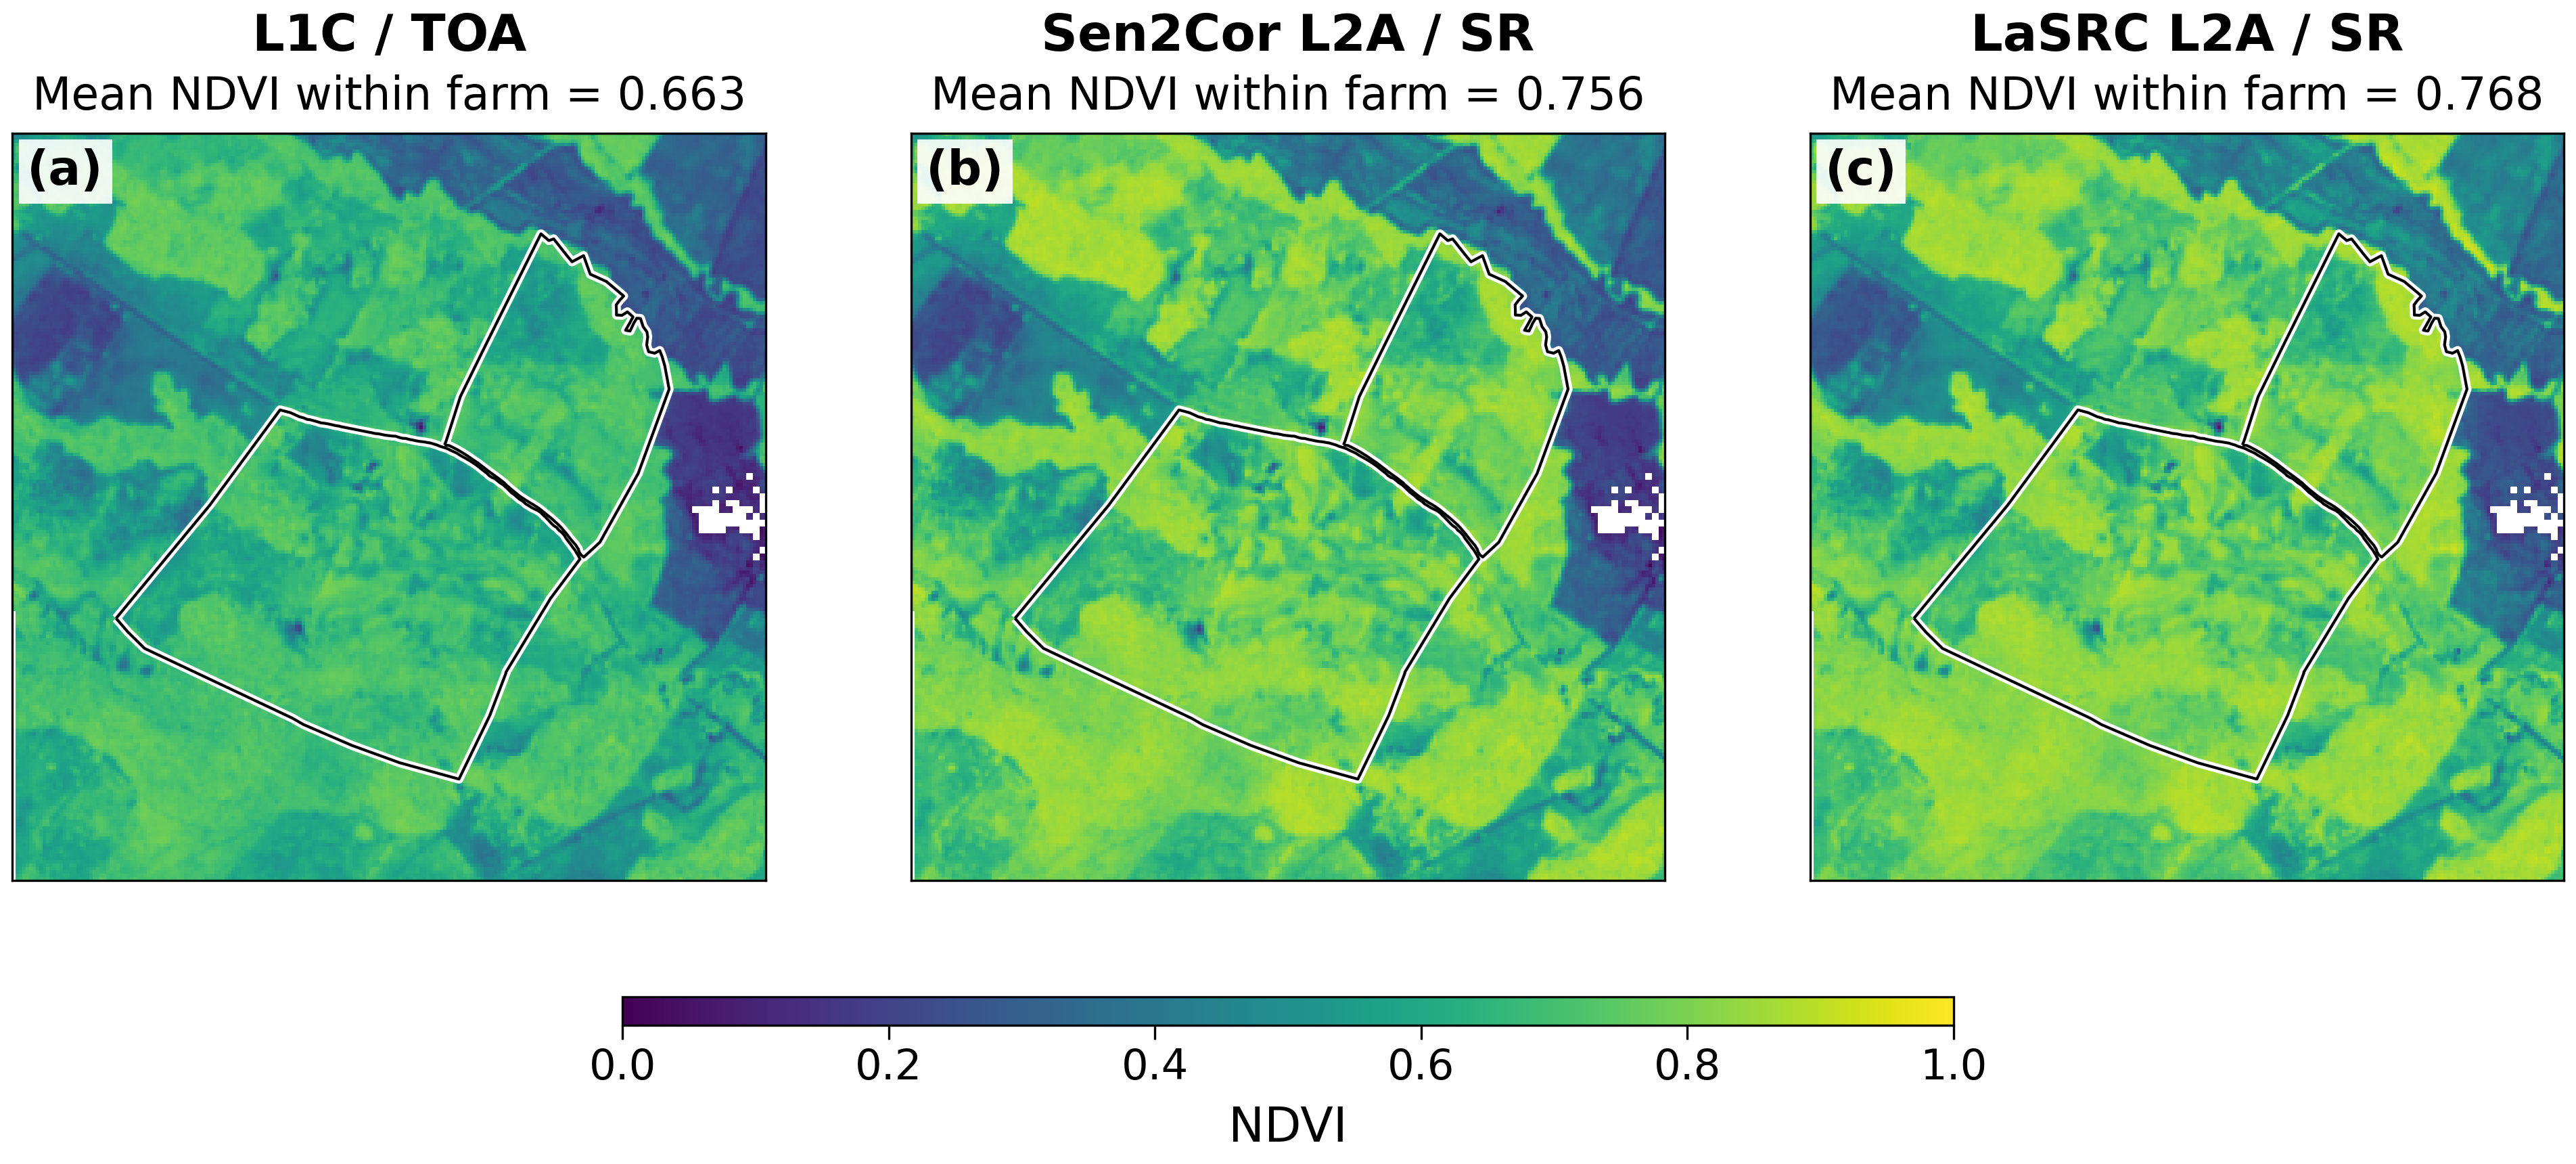
\includegraphics[width=1\textwidth,height=\textheight]{figures/figure_03_ndvi_comparison.png}

}

\caption{\label{fig-three-pipelines}Sentinel-2 NDVI for farm 3948 on 7
August 2019 across L1C/TOA, Sen2Cor L2A/SR, and LaSRC L2A/SR. The panels
share the same 10 m grid (L1C reference), a 300 m context around the
farm, and the same NDVI scale; only pixels valid in all three products
are shown. The outline marks the farm boundary, and the mean NDVI is
computed within it.}

\end{figure}%

For the illustrated acquisition, mean NDVI within farm 3948 increased
from 0.663 for L1C to 0.756 for Sen2Cor and 0.768 for LaSRC. The spatial
pattern was consistent among products, while the two SR pipelines
produced higher values over most vegetated pixels. This example
illustrates processor-associated differences but does not establish
absolute accuracy.

\subsection{Scene Availability and Comparison
Period}\label{sec-sen2cor-availability}

Sen2Cor observations were matched to acquisition dates already processed
in the local L1C/LaSRC inventory. Matching yielded 81 of 103 available
dates in 2019 and 94 of 114 dates in 2020, compared with no more than
eight matched dates per year during 2016-2018
(Table~\ref{tbl-sen2cor-availability}). The agreement analysis was
therefore restricted to 2019 and 2020.

\begin{longtable}[]{@{}
  >{\raggedleft\arraybackslash}p{(\columnwidth - 8\tabcolsep) * \real{0.2000}}
  >{\raggedleft\arraybackslash}p{(\columnwidth - 8\tabcolsep) * \real{0.2000}}
  >{\raggedleft\arraybackslash}p{(\columnwidth - 8\tabcolsep) * \real{0.2000}}
  >{\raggedleft\arraybackslash}p{(\columnwidth - 8\tabcolsep) * \real{0.2000}}
  >{\raggedleft\arraybackslash}p{(\columnwidth - 8\tabcolsep) * \real{0.2000}}@{}}
\caption{Sen2Cor date availability relative to the local L1C/LaSRC
inventory for Sentinel-2 tiles 18NXJ and
18NXK.}\label{tbl-sen2cor-availability}\tabularnewline
\toprule\noalign{}
\begin{minipage}[b]{\linewidth}\raggedleft
Image year
\end{minipage} & \begin{minipage}[b]{\linewidth}\raggedleft
Vector geometry
\end{minipage} & \begin{minipage}[b]{\linewidth}\raggedleft
LaSRC dates available
\end{minipage} & \begin{minipage}[b]{\linewidth}\raggedleft
Sen2Cor dates matched
\end{minipage} & \begin{minipage}[b]{\linewidth}\raggedleft
Coverage (\%)
\end{minipage} \\
\midrule\noalign{}
\endfirsthead
\toprule\noalign{}
\begin{minipage}[b]{\linewidth}\raggedleft
Image year
\end{minipage} & \begin{minipage}[b]{\linewidth}\raggedleft
Vector geometry
\end{minipage} & \begin{minipage}[b]{\linewidth}\raggedleft
LaSRC dates available
\end{minipage} & \begin{minipage}[b]{\linewidth}\raggedleft
Sen2Cor dates matched
\end{minipage} & \begin{minipage}[b]{\linewidth}\raggedleft
Coverage (\%)
\end{minipage} \\
\midrule\noalign{}
\endhead
\bottomrule\noalign{}
\endlastfoot
2016 & 2015 & 49 & 1 & 2.0 \\
2017 & 2015 & 72 & 1 & 1.4 \\
2018 & 2019 & 99 & 8 & 8.1 \\
2019 & 2019 & 103 & 81 & 78.6 \\
2020 & 2019 & 114 & 94 & 82.5 \\
\end{longtable}

\subsection{Three-Pipeline
Agreement}\label{sec-three-pipeline-agreement}

The common dataset contained 1,797 polygon-by-date observations from 106
polygons on 22 farms. Both SR pipelines produced systematically higher
NDVI than L1C (Table~\ref{tbl-agreement-3vias};
Figure~\ref{fig-agreement-3vias}). The LaSRC-L1C mean difference was
+0.116 (95\% CI, 0.108 to 0.124), with RMSD = 0.121 and uRMSD = 0.035;
the Sen2Cor-L1C mean difference was +0.095 (0.086 to 0.101), with RMSD =
0.101 and uRMSD = 0.034. In both comparisons, the mean shift accounted
for most of the total deviation, and the estimated Bland-Altman limits
of agreement were entirely above zero. The Deming slopes of 1.092 (1.050
to 1.122) and 1.155 (1.120 to 1.179) exceeded one, indicating that
neither TOA-SR relationship can be represented by a constant additive
shift alone.

\begin{longtable}[]{@{}lrrr@{}}
\caption{Agreement statistics for the common 2019-2020 polygon-by-date
dataset (N = 1,797; 106 polygons; 22 farms). Confidence intervals are
95\% farm-cluster bootstrap percentile intervals (2,000 replicates).
Differences are the first-named pipeline minus the second. All
statistics were calculated from unrounded values. LoA, Bland-Altman
limits of agreement.}\label{tbl-agreement-3vias}\tabularnewline
\toprule\noalign{}
Statistic & LaSRC-L1C & Sen2Cor-L1C & LaSRC-Sen2Cor \\
\midrule\noalign{}
\endfirsthead
\toprule\noalign{}
Statistic & LaSRC-L1C & Sen2Cor-L1C & LaSRC-Sen2Cor \\
\midrule\noalign{}
\endhead
\bottomrule\noalign{}
\endlastfoot
Mean difference & +0.116 & +0.095 & +0.021 \\
95\% CI & {[}0.108, 0.124{]} & {[}0.086, 0.101{]} & {[}0.016,
0.026{]} \\
RMSD & 0.121 & 0.101 & 0.036 \\
uRMSD & 0.035 & 0.034 & 0.029 \\
CCC & 0.653 & 0.743 & 0.962 \\
95\% CI & {[}0.576, 0.704{]} & {[}0.671, 0.796{]} & {[}0.948,
0.972{]} \\
\(R^2\) & 0.923 & 0.942 & 0.953 \\
Deming slope & 1.092 & 1.155 & 0.945 \\
95\% CI & {[}1.050, 1.122{]} & {[}1.120, 1.179{]} & {[}0.916,
0.972{]} \\
Deming intercept & +0.062 & +0.004 & +0.059 \\
95\% LoA & {[}+0.047, +0.184{]} & {[}+0.027, +0.162{]} & {[}-0.035,
+0.078{]} \\
\end{longtable}

\begin{figure}[htbp]

\centering{

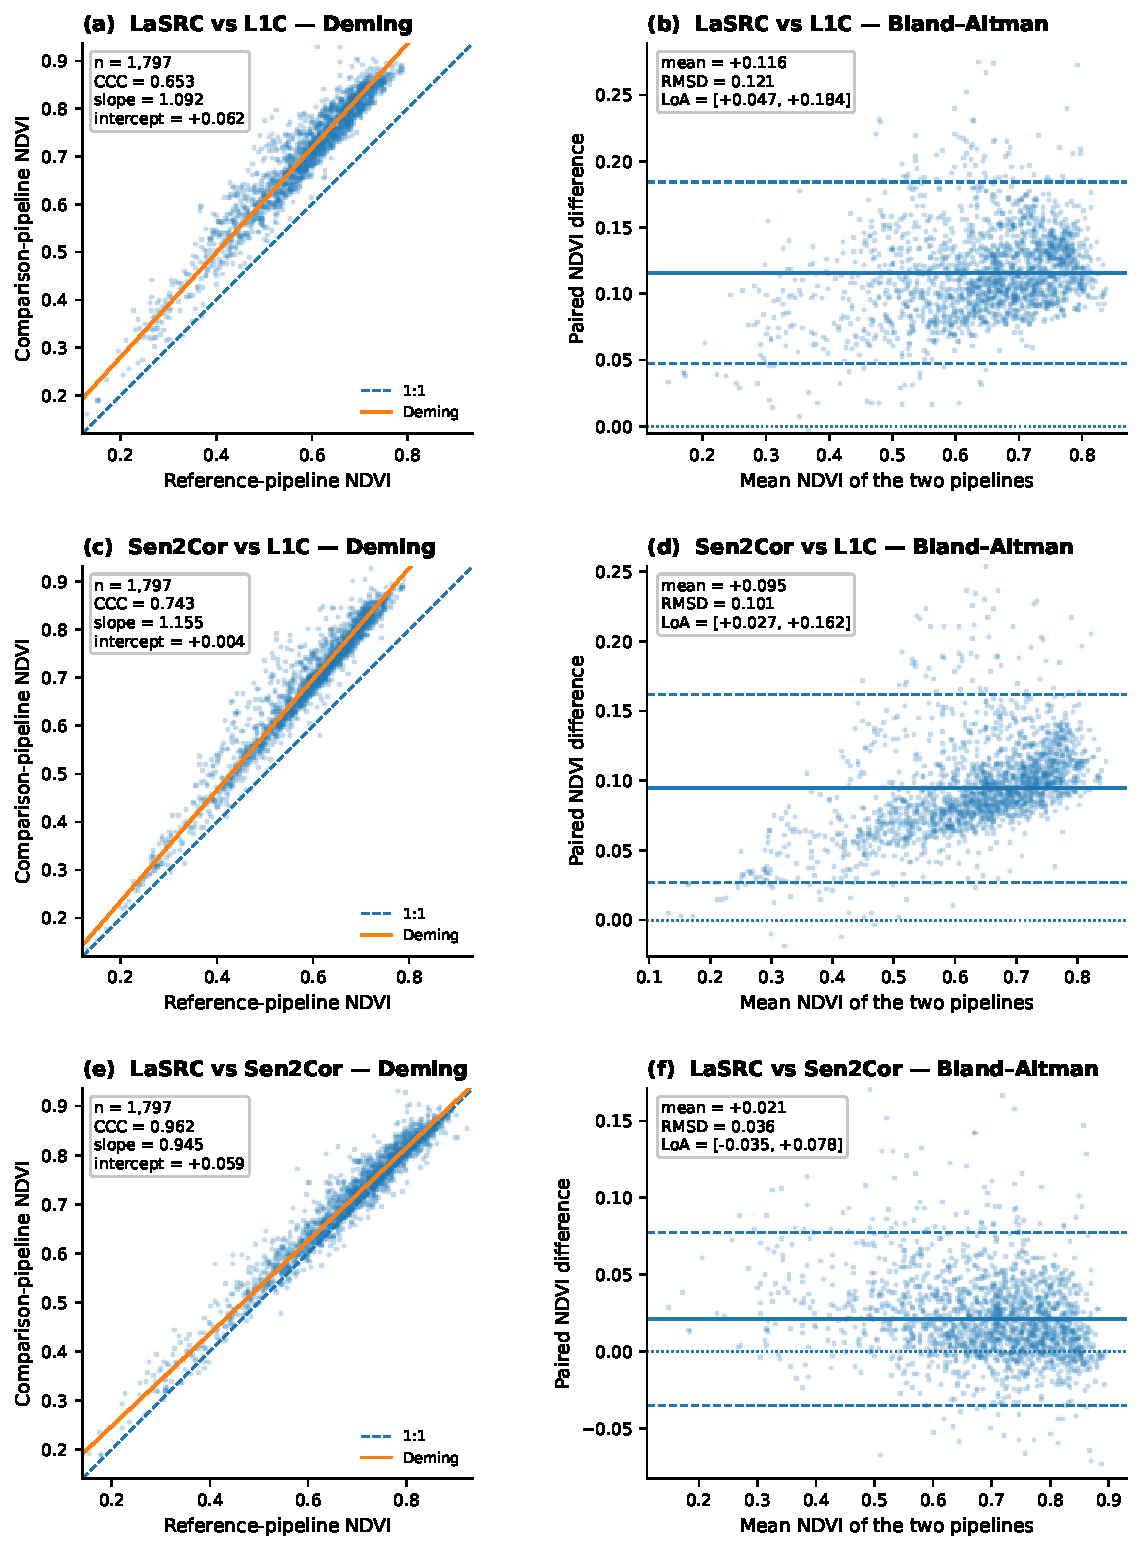
\includegraphics[width=0.94\textwidth,height=\textheight]{figures/figure_04_agreement_diagnostics.pdf}

}

\caption{\label{fig-agreement-3vias}Agreement diagnostics for the common
2019-2020 dataset. Rows compare LaSRC-L1C, Sen2Cor-L1C, and
LaSRC-Sen2Cor. Left panels show Deming regression and the 1:1 line;
right panels show Bland-Altman difference-versus-mean diagnostics.}

\end{figure}%

Agreement between the two SR pipelines was substantially stronger than
agreement between either SR pipeline and L1C. LaSRC-Sen2Cor had a mean
difference of +0.021, RMSD = 0.036, uRMSD = 0.029, and CCC = 0.962. The
Deming slope of 0.945, whose confidence interval (0.916 to 0.972)
excluded one, and the intercept of +0.059 indicate a small proportional
component, while the limits of agreement {[}-0.035, +0.078{]} show that
individual differences may occur in either direction. Thus, Sen2Cor and
LaSRC were closely concordant but not numerically interchangeable.

The same pattern was observed separately in each year
(Table~\ref{tbl-agreement-annual}). The LaSRC-Sen2Cor mean difference
was practically identical in 2019 (+0.021) and 2020 (+0.021), with
overlapping confidence intervals, and its Deming slope was below one in
both years. The TOA-SR mean differences were slightly larger in 2019
than in 2020, and CCC was lower in 2020 for all three comparisons. For
LaSRC-L1C in 2019, the Deming slope interval (0.996 to 1.084) included
one, so a proportional component was not distinguishable for that year
alone.

\begin{longtable}[]{@{}lrrrrr@{}}
\caption{Annual agreement statistics (106 polygons and 22 farms in each
year). Values in brackets below each estimate are 95\% farm-cluster
bootstrap percentile
intervals.}\label{tbl-agreement-annual}\tabularnewline
\toprule\noalign{}
Pair & Year & N & Mean difference & CCC & Deming slope \\
\midrule\noalign{}
\endfirsthead
\toprule\noalign{}
Pair & Year & N & Mean difference & CCC & Deming slope \\
\midrule\noalign{}
\endhead
\bottomrule\noalign{}
\endlastfoot
LaSRC-L1C & 2019 & 668 & +0.120 & 0.692 & 1.045 \\
& & & {[}0.111, 0.128{]} & {[}0.619, 0.751{]} & {[}0.996, 1.084{]} \\
LaSRC-L1C & 2020 & 1,129 & +0.114 & 0.616 & 1.144 \\
& & & {[}0.105, 0.122{]} & {[}0.509, 0.695{]} & {[}1.088, 1.191{]} \\
Sen2Cor-L1C & 2019 & 668 & +0.098 & 0.771 & 1.128 \\
& & & {[}0.087, 0.108{]} & {[}0.692, 0.835{]} & {[}1.071, 1.164{]} \\
Sen2Cor-L1C & 2020 & 1,129 & +0.092 & 0.716 & 1.189 \\
& & & {[}0.086, 0.098{]} & {[}0.624, 0.778{]} & {[}1.165, 1.213{]} \\
LaSRC-Sen2Cor & 2019 & 668 & +0.021 & 0.967 & 0.928 \\
& & & {[}0.017, 0.027{]} & {[}0.956, 0.975{]} & {[}0.903, 0.954{]} \\
LaSRC-Sen2Cor & 2020 & 1,129 & +0.021 & 0.957 & 0.959 \\
& & & {[}0.015, 0.027{]} & {[}0.934, 0.973{]} & {[}0.921, 0.989{]} \\
\end{longtable}

\subsection{Sensitivity to LaSRC Masking}\label{sec-masking-sensitivity}

Masking sensitivity was evaluated on the identical set of 2,585
observations (128 polygons, 20 farms) available in both LaSRC exports
(Table~\ref{tbl-mask-paired}). The masked-minus-unmasked change in mean
difference was +0.0001 (95\% farm-cluster bootstrap CI, -0.0021 to
0.0024), and the change in CCC was +0.0014 (-0.0078 to 0.0146). Both
intervals included zero. The Deming slope increased by +0.0191 (0.0028
to 0.0312), whose interval excluded zero, indicating a small but
statistically distinguishable change in the proportional relationship.
Restricting the comparison to the 2,521 records with at least 10 valid
pixels in both LaSRC exports gave the same conclusions: +0.0002 (-0.0021
to 0.0026) for the mean difference, +0.0019 (-0.0079 to 0.0160) for CCC,
and +0.0179 (0.0017 to 0.0297) for the Deming slope.

\begin{longtable}[]{@{}
  >{\raggedright\arraybackslash}p{(\columnwidth - 8\tabcolsep) * \real{0.2754}}
  >{\raggedleft\arraybackslash}p{(\columnwidth - 8\tabcolsep) * \real{0.1449}}
  >{\raggedleft\arraybackslash}p{(\columnwidth - 8\tabcolsep) * \real{0.1449}}
  >{\raggedleft\arraybackslash}p{(\columnwidth - 8\tabcolsep) * \real{0.1594}}
  >{\raggedleft\arraybackslash}p{(\columnwidth - 8\tabcolsep) * \real{0.2754}}@{}}
\caption{Paired masking comparison on 2,585 common polygon-by-date
observations (128 polygons; 20
farms).}\label{tbl-mask-paired}\tabularnewline
\toprule\noalign{}
\begin{minipage}[b]{\linewidth}\raggedright
Metric
\end{minipage} & \begin{minipage}[b]{\linewidth}\raggedleft
Masked LaSRC
\end{minipage} & \begin{minipage}[b]{\linewidth}\raggedleft
Unmasked LaSRC
\end{minipage} & \begin{minipage}[b]{\linewidth}\raggedleft
Difference (masked-unmasked)
\end{minipage} & \begin{minipage}[b]{\linewidth}\raggedleft
95\% farm-cluster bootstrap CI
\end{minipage} \\
\midrule\noalign{}
\endfirsthead
\toprule\noalign{}
\begin{minipage}[b]{\linewidth}\raggedright
Metric
\end{minipage} & \begin{minipage}[b]{\linewidth}\raggedleft
Masked LaSRC
\end{minipage} & \begin{minipage}[b]{\linewidth}\raggedleft
Unmasked LaSRC
\end{minipage} & \begin{minipage}[b]{\linewidth}\raggedleft
Difference (masked-unmasked)
\end{minipage} & \begin{minipage}[b]{\linewidth}\raggedleft
95\% farm-cluster bootstrap CI
\end{minipage} \\
\midrule\noalign{}
\endhead
\bottomrule\noalign{}
\endlastfoot
Mean difference relative to Sen2Cor & +0.020 & +0.020 & +0.0001 &
{[}-0.0021, +0.0024{]} \\
CCC & 0.954 & 0.953 & +0.0014 & {[}-0.0078, +0.0146{]} \\
Deming slope & 0.950 & 0.931 & +0.0191 & {[}+0.0028, +0.0312{]} \\
\end{longtable}

These results indicate that Fmask+s2cloudless screening did not
materially change the aggregate mean difference or concordance for
observations retained in both datasets, although it produced a small
change in the Deming slope.

\subsection{Differences among SCR Land-Use
Categories}\label{sec-gradiente-ut}

The category-stratified dataset comprised 1,527 observations from 88
polygons on 21 farms. Mean paired differences were positive in every
category and for all three comparisons (Table~\ref{tbl-gradiente-ut};
Figure~\ref{fig-gradiente-ut}). For LaSRC-L1C, category means ranged
from +0.095 in UT8 to +0.139 in UT2. For Sen2Cor-L1C, they ranged from
+0.076 in UT8 to +0.126 in UT2. The corresponding 95\% farm-cluster
bootstrap intervals for UT2 and UT8 did not overlap in either TOA-SR
comparison. Because a direct UT2-UT8 contrast was not estimated and some
categories were represented by only two to four farms, the pattern is
interpreted as category-associated variation rather than as a formal
pairwise hypothesis test.

\begin{longtable}[]{@{}
  >{\raggedright\arraybackslash}p{(\columnwidth - 12\tabcolsep) * \real{0.0946}}
  >{\raggedleft\arraybackslash}p{(\columnwidth - 12\tabcolsep) * \real{0.0676}}
  >{\raggedleft\arraybackslash}p{(\columnwidth - 12\tabcolsep) * \real{0.0676}}
  >{\raggedleft\arraybackslash}p{(\columnwidth - 12\tabcolsep) * \real{0.0946}}
  >{\raggedleft\arraybackslash}p{(\columnwidth - 12\tabcolsep) * \real{0.2162}}
  >{\raggedleft\arraybackslash}p{(\columnwidth - 12\tabcolsep) * \real{0.2162}}
  >{\raggedleft\arraybackslash}p{(\columnwidth - 12\tabcolsep) * \real{0.2432}}@{}}
\caption{Mean paired NDVI differences by SCR land-use category for
2019-2020 (1,527 observations; 88 polygons; 21 farms). N,
polygon-by-date observations; the last three columns are mean
differences (first-named pipeline minus the second). Category labels are
given in Table~\ref{tbl-ut}. The 95\% farm-cluster bootstrap intervals
are shown in
Figure~\ref{fig-gradiente-ut}.}\label{tbl-gradiente-ut}\tabularnewline
\toprule\noalign{}
\begin{minipage}[b]{\linewidth}\raggedright
Category
\end{minipage} & \begin{minipage}[b]{\linewidth}\raggedleft
N
\end{minipage} & \begin{minipage}[b]{\linewidth}\raggedleft
Farms
\end{minipage} & \begin{minipage}[b]{\linewidth}\raggedleft
Polygons
\end{minipage} & \begin{minipage}[b]{\linewidth}\raggedleft
LaSRC-L1C
\end{minipage} & \begin{minipage}[b]{\linewidth}\raggedleft
Sen2Cor-L1C
\end{minipage} & \begin{minipage}[b]{\linewidth}\raggedleft
LaSRC-Sen2Cor
\end{minipage} \\
\midrule\noalign{}
\endfirsthead
\toprule\noalign{}
\begin{minipage}[b]{\linewidth}\raggedright
Category
\end{minipage} & \begin{minipage}[b]{\linewidth}\raggedleft
N
\end{minipage} & \begin{minipage}[b]{\linewidth}\raggedleft
Farms
\end{minipage} & \begin{minipage}[b]{\linewidth}\raggedleft
Polygons
\end{minipage} & \begin{minipage}[b]{\linewidth}\raggedleft
LaSRC-L1C
\end{minipage} & \begin{minipage}[b]{\linewidth}\raggedleft
Sen2Cor-L1C
\end{minipage} & \begin{minipage}[b]{\linewidth}\raggedleft
LaSRC-Sen2Cor
\end{minipage} \\
\midrule\noalign{}
\endhead
\bottomrule\noalign{}
\endlastfoot
UT2 & 129 & 4 & 6 & +0.139 & +0.126 & +0.013 \\
UT3 & 471 & 14 & 28 & +0.136 & +0.109 & +0.027 \\
UT4 & 68 & 3 & 3 & +0.114 & +0.094 & +0.021 \\
UT7 & 36 & 2 & 3 & +0.108 & +0.099 & +0.009 \\
UT6 & 567 & 17 & 32 & +0.109 & +0.088 & +0.021 \\
UT8 & 256 & 10 & 16 & +0.095 & +0.076 & +0.019 \\
\end{longtable}

\begin{figure}[htbp]

\centering{

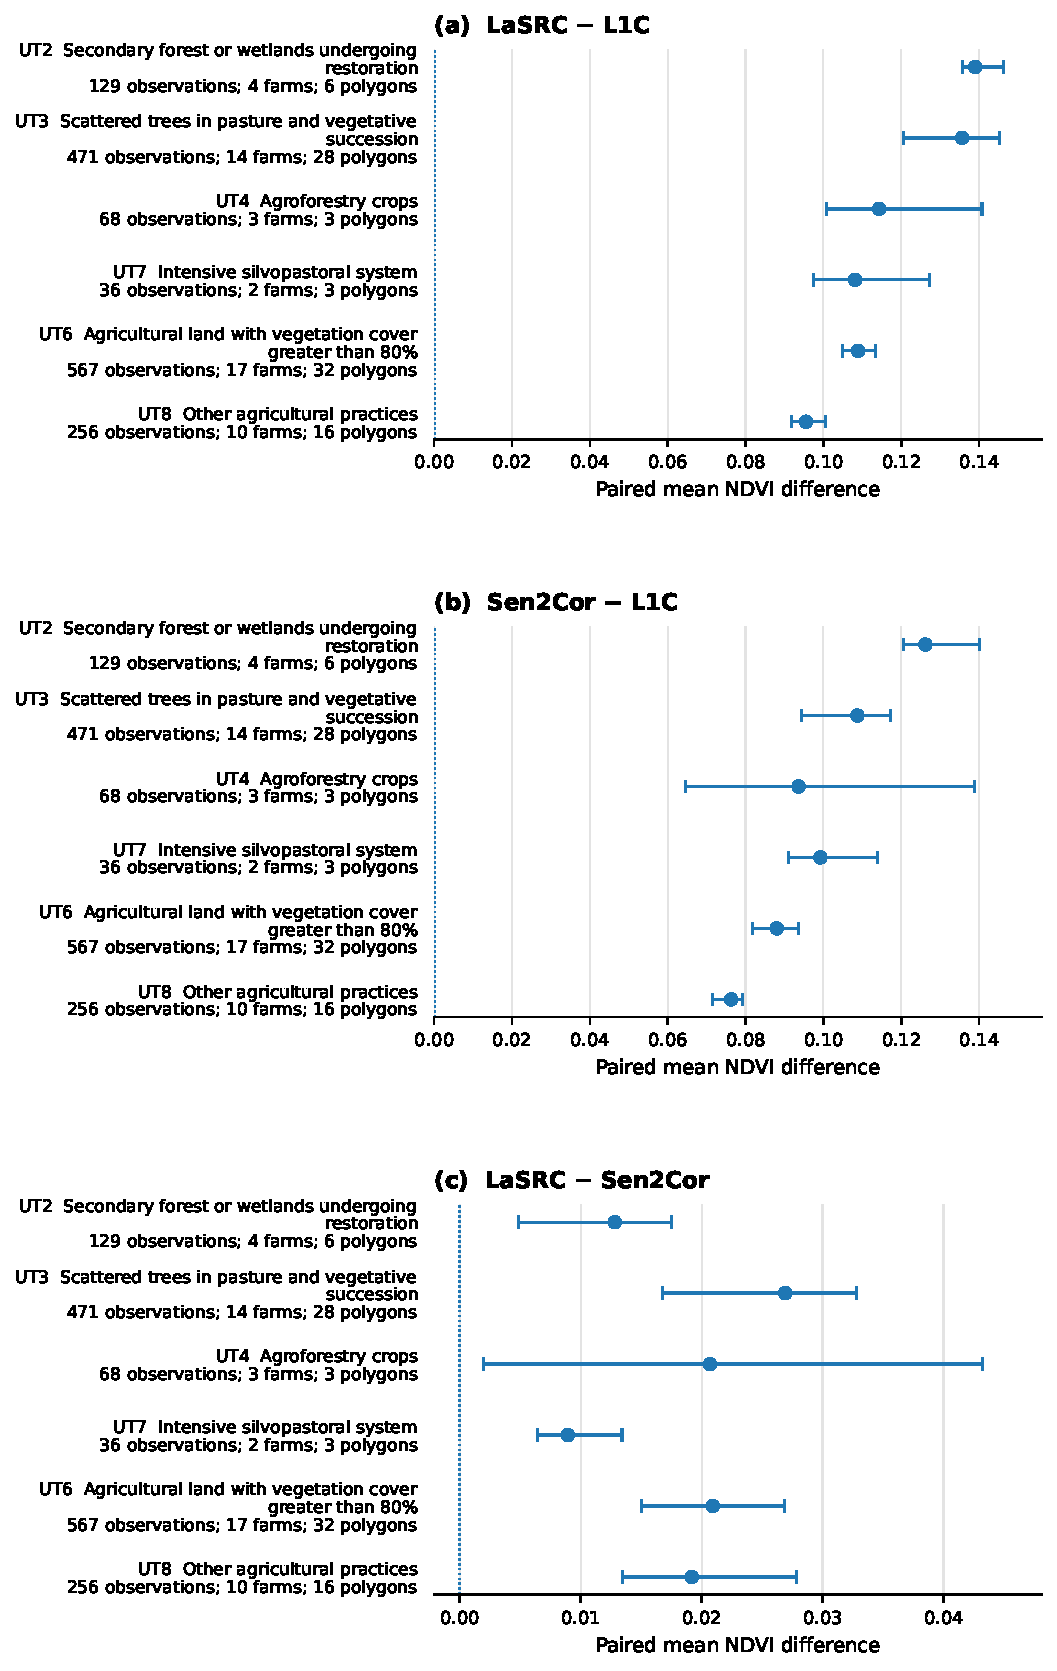
\includegraphics[width=0.92\textwidth,height=\textheight]{figures/figure_05_land_use_gradient.pdf}

}

\caption{\label{fig-gradiente-ut}Mean paired NDVI differences and 95\%
farm-cluster bootstrap intervals by SCR land-use category. Panels
compare LaSRC-L1C, Sen2Cor-L1C, and LaSRC-Sen2Cor; labels report the
numbers of observations, farms, and polygons.}

\end{figure}%

The LaSRC-Sen2Cor differences were smaller and varied over a narrower
range (+0.009 to +0.027) than either TOA-SR comparison. Their ordering
across categories differed from the TOA-SR pattern, indicating that
land-use dependence was not identical for all three processor pairs.

\section{Discussion}\label{sec-discussion}

\subsection{Inter-Processor Agreement}\label{sec-disc-agreement}

The two atmospheric-correction pipelines changed NDVI in the same
general direction relative to L1C, but the magnitude and proportional
structure differed. The positive mean differences and positive
Bland-Altman limits for LaSRC-L1C and Sen2Cor-L1C show that SR-derived
NDVI was consistently higher than TOA-derived NDVI in this dataset. The
low uRMSD relative to RMSD indicates that systematic displacement,
rather than random pairwise dispersion, accounted for most of the TOA-SR
disagreement. Nevertheless, Deming slopes above one demonstrate an
NDVI-dependent component, so a single additive adjustment would not
reproduce either SR series across the observed range.

Sen2Cor and LaSRC showed high concordance (CCC = 0.962) and a much
smaller mean difference and RMSD than either comparison with L1C. This
close agreement is consistent with both processors removing a
substantial common atmospheric component. However, the Deming slope of
0.945, non-zero intercept, and limits of agreement spanning negative and
positive values show that the two SR products are not equivalent at the
polygon-by-date level. The near-identical LaSRC-Sen2Cor mean difference
in 2019 and 2020, together with Deming slopes below one in both years,
suggests that this residual offset was stable over the study period
rather than driven by a single year.

The residual LaSRC-Sen2Cor differences cannot be assigned to a single
algorithmic source. Plausible contributors include the atmospheric
auxiliary data, aerosol and water-vapour retrievals, radiative-transfer
parameterization, cloud-screening implementation, rasterization, and
observation geometry \citep{MainKnorn2017, Vermote2016, Vermote2018}.
Because the LaSRC output analysed here was not an HLS NBAR product, BRDF
normalization is not attributed to LaSRC itself
\citep{Franch2019, USGSHLS2024}.

\subsection{Land-Use Dependence}\label{sec-disc-gradiente}

The largest TOA-SR differences occurred in UT2, which comprises
secondary forest or wetlands undergoing restoration, whereas the
smallest occurred in UT8, which comprises other agricultural practices.
This pattern is consistent with land-use-dependent differences in canopy
structure, shadow fraction, and red and near-infrared spectral response.
However, these mechanisms were not isolated experimentally, and the
limited number of farms in UT2, UT4, and UT7 constrains the precision of
category-level inference.

The narrower and differently ordered LaSRC-Sen2Cor differences indicate
that much of the category-associated TOA-SR pattern was common to both
atmospheric-correction pipelines. The remaining SR-SR variation was
comparatively small and should be interpreted as a residual processor
effect rather than as evidence of a uniform category correction.

\subsection{Masking Sensitivity}\label{sec-disc-masking}

On the paired observation set, Fmask+s2cloudless screening produced no
statistically distinguishable change in the aggregate mean difference or
CCC, because both cluster-bootstrap intervals included zero. The small
increase in Deming slope was statistically distinguishable from zero,
indicating that screening modified the proportional relationship more
than the average offset. In this analysis, masking therefore operated
primarily as pixel-quality selection rather than as a direct radiometric
adjustment of the retained polygon means.

\subsection{Limitations}\label{sec-limitations}

First, the farms form a spatially clustered observational sample within
one tropical landscape, so the numerical estimates should not be
generalized without independent replication. Second, the absence of
co-located field spectroradiometry or atmospheric reference measurements
prevents assessment of absolute processor accuracy. Third, the Sen2Cor
and local pipelines used different cloud-screening and aggregation
environments, so the processing-chain effect cannot be attributed
exclusively to atmospheric correction. Fourth, no explicit BRDF
normalization was applied. Fifth, one observation was removed through
data-dependent quality control; a pre-specified exclusion rule would
provide stronger protection against analytical discretion. Sixth, the
farm-cluster bootstrap preserves dependence among dates and among
polygons within farms, but no explicit hierarchical model was fitted,
and several land-use categories are represented by few farms. Seventh,
records of two inventory features that shared the same polygon
identifier, and polygon-by-date records duplicated within a pipeline,
were excluded rather than reconciled. Finally, the Earth Engine notebook
used for the final Sen2Cor export was not preserved; the SCL screening
rule is therefore documented from an earlier version of the extraction
code and from the structure of the exported records.

\subsection{Implications for Multi-Year NDVI
Analysis}\label{sec-outlook}

Sentinel-2 time series that combine L1C and SR observations should not
assume that the products differ only by a constant offset. Harmonization
should account for both systematic and proportional differences and
should be validated within the target landscape and land-use
composition. Future comparisons should apply a common pixel mask and
grid to locally processed outputs, fit hierarchical models of dates,
polygons, and farms, include an external atmospheric or surface
reference, and evaluate additional years and independent tropical
landscapes.

\section{Conclusions}\label{sec-conclusions}

Across 1,797 common polygon-by-date observations from 106 management
polygons on 22 farms in 2019 and 2020, LaSRC and Sen2Cor produced higher
NDVI than L1C by mean paired differences of +0.116 and +0.095,
respectively. The corresponding Deming slopes of 1.092 and 1.155 show
that these differences contained both systematic and proportional
components.

Agreement between the SR products was markedly stronger (mean difference
= +0.021; RMSD = 0.036; CCC = 0.962), and the mean difference was stable
between years, although the Deming slope of 0.945 and limits of
agreement from -0.035 to +0.078 show that Sen2Cor and LaSRC were not
interchangeable for individual polygon-date observations.

The TOA-SR differences varied among SCR land-use categories, with the
largest values in secondary forest or wetlands undergoing restoration
and the smallest in other agricultural practices. On the paired masking
subset, the mean difference and CCC were statistically stable, whereas
the Deming slope changed slightly. These findings support explicit,
locally validated harmonization when Sentinel-2 NDVI series combine TOA
and SR products or multiple atmospheric-correction processors.

\section*{Author Contributions}\label{author-contributions}
\addcontentsline{toc}{section}{Author Contributions}

Conceptualization, methodology, software, validation, formal analysis,
investigation, data curation, visualization, writing---original draft
preparation, and writing---review and editing, H.A.P.V. The author has
read and agreed to the published version of the manuscript.

\section*{Funding}\label{funding}
\addcontentsline{toc}{section}{Funding}

This research received no direct external funding.

\section*{Institutional Review Board
Statement}\label{institutional-review-board-statement}
\addcontentsline{toc}{section}{Institutional Review Board Statement}

Not applicable. The study used satellite imagery and an existing
geospatial land-use inventory and did not involve human participants or
animals.

\section*{Informed Consent Statement}\label{informed-consent-statement}
\addcontentsline{toc}{section}{Informed Consent Statement}

Not applicable.

\section*{Data Availability
Statement}\label{data-availability-statement}
\addcontentsline{toc}{section}{Data Availability Statement}

The derived statistical tables, analysis code, input-scene and
auxiliary-data manifests, and computational-environment records are
openly available in Zenodo at {[}ZENODO DOI --- to be assigned at
release{]}. The LaSRC processing image is the \texttt{lasrc-fmask} image
of the \texttt{sen2lasrc} GitLab registry
(registry.gitlab.com/floriandeboissieu/sen2lasrc), pinned by SHA-256
digest \texttt{14fcc58ac2bd…}; the full digest is recorded in the Zenodo
deposit. Sentinel-2 Level-1C and Level-2A products are available from
the Copernicus Data Space Ecosystem and Google Earth Engine.
Farm-boundary and management-polygon geometries are subject to the
data-governance conditions of the Sustainable Cattle Ranching project
and are therefore not publicly distributed; their identity and
processing are documented in the deposited geometry manifest.

\section*{Acknowledgments}\label{acknowledgments}
\addcontentsline{toc}{section}{Acknowledgments}

The author acknowledges the Sustainable Cattle Ranching project
partnership---FEDEGÁN-FNG, CIPAV, Fondo Acción, The Nature Conservancy,
and the World Bank---for the institutional and technical work that
produced the land-use classification framework and the 2019 polygon
inventory used in this study. The author also thanks USGS EROS User
Services for access to atmospheric auxiliary data and Florian de
Boissieu and contributors for developing and maintaining
\texttt{sen2lasrc}. During the preparation of this manuscript, the
author used Claude (Anthropic; most recently Opus 5.5) and ChatGPT
(OpenAI; most recently GPT-6 and GPT-5.6 Sol) between January and
October 2026 for the purposes described in Section~\ref{sec-genai}. The
author has reviewed and edited the output and takes full responsibility
for the content of this publication.

\section*{Conflicts of Interest}\label{conflicts-of-interest}
\addcontentsline{toc}{section}{Conflicts of Interest}

The author declares no conflicts of interest.

\section*{Abbreviations}\label{abbreviations}
\addcontentsline{toc}{section}{Abbreviations}

\begin{longtable}[]{@{}
  >{\raggedright\arraybackslash}p{(\columnwidth - 2\tabcolsep) * \real{0.5000}}
  >{\raggedright\arraybackslash}p{(\columnwidth - 2\tabcolsep) * \real{0.5000}}@{}}
\toprule\noalign{}
\begin{minipage}[b]{\linewidth}\raggedright
Abbreviation
\end{minipage} & \begin{minipage}[b]{\linewidth}\raggedright
Meaning
\end{minipage} \\
\midrule\noalign{}
\endhead
\bottomrule\noalign{}
\endlastfoot
AOI & Area of interest \\
AOT & Aerosol optical thickness \\
BRDF & Bidirectional reflectance distribution function \\
CCC & Lin's concordance correlation coefficient \\
CI & Confidence interval \\
GEE & Google Earth Engine \\
HLS & Harmonized Landsat Sentinel-2 \\
LoA & Limits of agreement \\
MSI & MultiSpectral Instrument \\
NBAR & Nadir BRDF-adjusted reflectance \\
NDVI & Normalized Difference Vegetation Index \\
RMSD & Root-mean-square deviation \\
SCL & Scene Classification Layer \\
SCR & Sustainable Cattle Ranching project (\emph{Proyecto Ganadería
Colombiana Sostenible}) \\
SR & Surface reflectance \\
TOA & Top-of-atmosphere \\
uRMSD & Unbiased root-mean-square deviation \\
UT & Land-use category code in the SCR classification \\
\end{longtable}

\begin{adjustwidth}{-\extralength}{0cm}
\reftitle{References}
\bibliography{references-v12}
\end{adjustwidth}

\end{document}
